\documentclass[semifinal]{cpecmu}

%% This is a sample document demonstrating how to use the CPECMU
%% project template. If you are having trouble, see "cpecmu.pdf" for
%% documentation.

\projectNo{S021-1/65}
\acadyear{2022}

\titleTH{เว็ปไซต์สร้าง และจัดการทัวร์นาเมนต์}
\titleEN{Website For Organize and Manage Tournaments}

\author{นายภูเบศ รุจิเรกานุสรณ์}{Phubet Rujirekanusorn}{620610804}


\cpeadvisor{juggapong}
\cpecommittee{trasapong}
\cpecommittee{navadon}

%% Some possible packages to include:
\usepackage[final]{graphicx} % for including graphics

%% Add bookmarks and hyperlinks in the document.
\PassOptionsToPackage{hyphens}{url}
\usepackage[colorlinks=true,allcolors=Blue4,citecolor=red,linktoc=all]{hyperref}
\def\UrlLeft#1\UrlRight{$#1$}

%% Needed just by this example, but maybe not by most reports
\usepackage{afterpage} % for outputting
\usepackage{pdflscape} % for landscape figures and tables. 

%% Some other useful packages. Look these up to find out how to use
%% them.
% \usepackage{natbib}    % for author-year citation styles
% \usepackage{txfonts}
% \usepackage{appendix}  % for appendices on a per-chapter basis
% \usepackage{xtab}      % for tables that go over multiple pages
% \usepackage{subfigure} % for subfigures within a figure
% \usepackage{pstricks,pdftricks} % for access to special PostScript and PDF commands
% \usepackage{nomencl}   % if you have a list of abbreviations

%% if you're having problems with overfull boxes, you may need to increase
%% the tolerance to 9999
% \tolerance=9999

\bibliographystyle{plain}
% \bibliographystyle{IEEEbib}

% \renewcommand{\topfraction}{0.85}
% \renewcommand{\textfraction}{0.1}
% \renewcommand{\floatpagefraction}{0.75}

%% Example for glossary entry
%% Need to use glossary option
%% See glossaries package for complete documentation.
\ifglossary
  \newglossaryentry{lorem ipsum}{
    name=lorem ipsum,
    description={derived from Latin dolorem ipsum, translated as ``pain itself''}
  }
\fi

%% Uncomment this command to preview only specified LaTeX file(s)
%% imported with \include command below.
%% Any other file imported via \include but not specified here will not
%% be previewed.
%% Useful if your report is large, as you might not want to build
%% the entire file when editing a certain part of your report.
% \includeonly{chapters/intro,chapters/background}

\begin{document}
\maketitle
\makesignature

\ifproject
\begin{abstractTH}


    โครงงานนี้ได้นำเสนอเว็บไซต์ที่ใช้ในการให้บริการ จัดสร้าง และจัดการทัวร์นาเมนต์ที่ครบจบในที่เดียว อีกทั้งยังมีระบบในการเก็บประวัติให้แก่ผู้เล่นให้นำไปใช้เป็นที่สะสมผลงาน และนำไปสานต่อในการเป็นผู้เล่น E-sport ในอนาคต
โดยเว็บไซต์ฝั่ง Frontend จะถูกพัฒนาด้วย React framework ใช้ภาษา JavaScript ฝั่ง Backend 
จะถูกพัฒนาด้วย Nest framework ใช้ภาษา TypeScript ในส่วนของฐานข้อมูลใช้การจัดเก็บข้อมูลแบบSQL ร่วมกับ PostgreSQL ในการจัดการ 
และใช้ Google Firebase Cloud Storage ในการจัดเก็บรูปภาพ
\end{abstractTH}

\begin{abstract}

    This project presents a website that can be used to serve, organize and manage tournament all in one website.
there is also a system to collect history for player to use as portfolio.And lead to future participation in E-sport Career.
The website's Forntend site will be developed with React framework using JavaScript. On the Backend site will be developed with Nest using TypeScript.For the database use SQL for storage with PostgreSQL
and Google Firebase Cloud Storage to store images.
\end{abstract}

\iffalse
\begin{dedication}
This document is dedicated to all Chiang Mai University students.

Dedication page is optional.
\end{dedication}
\fi % \iffalse



\contentspage

\ifproject
\figurelistpage

% \tablelistpage
\fi % \ifproject

% \abbrlist % this page is optional

% \symlist % this page is optional

% \preface % this section is optional


\pagestyle{empty}\cleardoublepage
\normalspacing \setcounter{page}{1} \pagenumbering{arabic} \pagestyle{cpecmu}

\chapter{\ifenglish Introduction\else บทนำ\fi}

\section{\ifenglish Project rationale\else ที่มาของโครงงาน\fi}
เนื่องจากการแข่งขัน E-sport กำลังเติบโตเป็นอย่างมากและเป็นที่นิยมขึ้นเรื่อยๆ ในการจัดการแข่งขันทัวร์นาเมนต์นั้น
ต้องใช้หลายแอพพลิเคชันในการจัดการทั้งใช้ในการจัดการคน การทำตารางแข่ง การเก็บบันทึกผล และการแสดงผลลัพธ์ ซึ่งต้องใช้
แอพพลิเคชันหลายอัน เช่น Excel, Photoshop และ Google Dirve   จึงเป็นที่มาของโครงงานนี้ที่จะนำสิ่งต่างๆที่จำเป็นมาไว้ในเว็ปไซต์นี้เว็ปไซต์เดียว
และ อีกหนึ่งเหตุผลก็คือต้องการยกระดับวงการ E-sport และให้โอกาศแก่ผู้ที่ต้องการเริ่มต้นเข้าสู่วงการที่ไม่ได้มีทุนมากมาย แต่มีใจที่จะมาสายงานนี้  


\section{\ifenglish Objectives\else วัตถุประสงค์ของโครงงาน\fi}
\begin{enumerate}
    \item พัฒนาเว็บแอพพลิเคชันที่ใช้ในการจัดสร้าง และจัดการทัวร์นาเมนต์ ได้ในที่เดียว
    \item ใช้เป็นที่เก็บผลงานของเหล่านักกีฬา E-sport ได้
    \item สามารถนำไปใช้ต่อยอดได้ในอนาคต
\end{enumerate}

\section{\ifenglish Project scope\else ขอบเขตของโครงงาน\fi}

\subsection{\ifenglish Software scope\else ขอบเขตด้านซอฟต์แวร์\fi}
\begin{enumerate}
    \item การสร้างทัวร์นาเมนต์จะมีแค่แบบเดียวคือ Double-elimination tournament \cite{tournament}
    \item สร้างทัวร์นาเมนต์จากเกมที่มีในระบบได้เท่านั้น 
    \item สามรถจัดเก็บประวัติ และจัดการโปรไฟล์ได้ตามที่มีกำหนดให้เท่านั้น
    \item การกำหนดผลการแข่งขั้นนั้นขึ้นอยู่กับผู้จัดการแข่งขันเป็นผู้จัดการไม่สามรถตรวจสอบเพื่อยืนยันได้
    \item ระบบความปลอดภัยขอเว็ปไซต์ใช้เพียงแค่ Token เท่านั้น
\end{enumerate}

\section{\ifenglish Expected outcomes\else ประโยชน์ที่ได้รับ\fi}
\begin{enumerate}
    \item ช่วยอำนวยความสะดวกให้ผู้ดูแลการแข่งขัน
    \item เป็นที่เก็บผลงานประวัติการแข่งขัน
    \item สามารถนำไปใช้ร่วมกับโปรเจค StartUp ของทีมผมเพื่อสร้าง Ecosystem ของวงการ E-sport
\end{enumerate}

\section{\ifenglish Technology and tools\else เทคโนโลยีและเครื่องมือที่ใช้\fi}

\subsection{\ifenglish Software technology\else เทคโนโลยีด้านซอฟต์แวร์\fi}
\begin{enumerate}
    \item React\cite{react} - Open-source Fontend library ของ JavaScript เพื่อใช้สร้างหน้า User Interface
    \item JavaScript\cite{javascript} - ภาษาโปรแกรมมิ่งที่ใช้ในการเขียนหน้าเว็ปไซต์
    \item Nest\cite{nest} - Progressive Framework สำหรับการสร้างแอพพลิเคชันสวน Backend ที่มีประสิทธิภาพ มีความน่าเชื่อถือ และสามารถขยายได้
    \item TypeScript\cite{typescript} - ภาษาโปรแกรมมิ่งที่มีความเคร่งครัดในชนิดของตัวแปลที่พัฒนามาจาก Javascript
    \item PostgreSQL\cite{postgresql} - ระบบการจัดการฐานข้อมูล object-relational โดยสามารถใช้รูปแบบคำสั่งของภาษา SQL
    \item Firebase Cloud Storage\cite{firebase} - Clound Storage สำหรับจัดเก็บข้อมูลเพื่อใช้ในการแสดง content เช่นรูป และ วีดีโอ
    \item Docker\cite{docker} - แพลตฟอร์มซอฟต์แวร์ที่ใช้ในการสร้าง Docker image และDocker Container 
\end{enumerate}

\section{\ifenglish Project plan\else แผนการดำเนินงาน\fi}

\begin{plan}{9}{2022}{2}{2023}
    \planitem{9}{2022}{10}{2022}{ออกแบบUX/UI เลือกเครื่องมือ และเขียนรายงาน}
    \planitem{10}{2022}{11}{2022}{พัฒนาฐานข้อมูล}
    \planitem{11}{2022}{2}{2023}{พัฒนาเว็ปแอพพลิเคชัน}
    \planitem{11}{2022}{2}{2023}{ทดสอบ}
    \planitem{2}{2023}{2}{2023}{Deploy web hosting}
    \planitem{2}{2023}{2}{2023}{จัดเตรียมนำเสนอ และสรุปผล}
\end{plan}
\begin{center}
**ทำการเปลี่ยนหัวข้อโปรเจคเมื่อวันที่ 24 ก.ย. 2565**
\end{center}

\section{\ifenglish%
Impacts of this project on society, health, safety, legal, and cultural issues
\else%
ผลกระทบด้านสังคม สุขภาพ ความปลอดภัย กฎหมาย และวัฒนธรรม
\fi}

ในการทำโครงงานนี้คาดว่าจะช่วยลดขั้นตอน และความยุ่งยากในการจัดสร้าง และจัดการทัวร์นาเมนต์
มากไปกว่านั้นเว็ปไซต์นี้จะเป็นศูนร่วมของเหล่านักกีฬา E-sport และเหล่าผู้จัดงาน ในอานาคต

\chapter{\ifenglish Background Knowledge and Theory\else ทฤษฎีที่เกี่ยวข้อง\fi}

การทำโครงงาน เริ่มต้นด้วยการศึกษาค้นคว้า ทฤษฎีที่เกี่ยวข้อง หรือ งานวิจัย/โครงงาน ที่เคยมีผู้นำเสนอไว้แล้ว ซึ่งเนื้อหาในบทนี้ก็จะเกี่ยวกับการอธิบายถึงสิ่งที่เกี่ยวข้องกับโครงงาน เพื่อให้ผู้อ่านเข้าใจเนื้อหาในบทถัดๆ ไปได้ง่ายขึ้น


\section{UX Design}
UX Design(User Experience Design) คือ การออกแบบเพื่อให้ผู้ใช้งานมีประสบการณ์ในการใช้งานที่ดีในเว็ปไซต์ หรือแอพพลิเคชันนั้นๆ
ไม่ว่าจะเป็นความง่ายในการใช้งาน ความต่อเนื่องในการใช้งาน การสื่อความหมาย ฯลฯ ตาม UX Law\cite{uxlaw} เพื่อประสบการณ์การที่ดีที่สุดของผู้ใช้งาน

\section{เครื่องมือที่ใช้ในการพัฒนา}
\subsection{React}
React เป็น Framework ที่ใช้งานกับ JavaScript ในการสร้างหน้า Fontend โดย React นั้นสามารถจัดการกับความซับซ้อนของระบบการทำงานได้โดยจะแบ่งส่วนการทำงานต่างๆออกจากกัน
เป็นส่วนเล็กๆที่สามารถจัดการได้ง่าย เช่น ส่วนของการแสดงผล ส่วนของงการทำงาน และในส่วนของการจัดการตัวแปร และในแต่ละส่วนก็จะแยกออกเป็นแต่ละระบบ เช่น ระบบล็อกอิน ระบบแดชบอร์ด ระบบจัดการสร้างทัวร์นาเมนต์ ฯลฯ 
ทำให้การจัดการนั้นง่าย และมีประสิทธิภาพ เนื่องจากเราสามารถรู้ได้ว่าจุดไหนมีปัญหาในการการทำงาน โค้ดสามารถอ่านได้ง่ายไม่เยอะจนเกินไป หลังจากนั้นค่อยนำมารวมกันโดยเรียกใช้ส่วนนั้นๆ และ React ยังมีตัวช่วยในการจัดการกับ State การทำงานของระบบ และจัดการกับ DOM
เมื่อมีการเปลี่ยนแปลงของข้อมูลใน DOM ได้ทันที และมากไปกว่านั้น React ได้ถูกใช้งานมาเป็นเวลานานทำให้มี UI Library ให้ใช้งานในการแสดงผลหน้าเว็ป และยังมีแหล่งข้อมูลในการหาความรู้ในการพัฒนาระบบเป็นจำนวนมากทำให้ง่าย และร่วดเร็วในการพัฒนาแพรตฟอร์มขึ้นเป็นอย่างมาก 

\begin{figure}[h]
    \begin{center}
    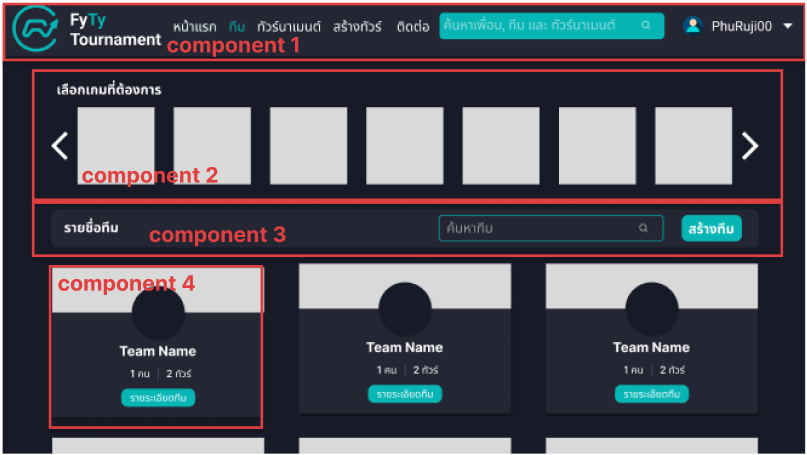
\includegraphics[width=10cm,height=10cm,keepaspectratio]{component.png}
    \end{center}
    \caption[การแยกส่วนต่างๆเป็น Component]{การแยกส่วนต่างๆเป็น Component}
    \label{fig:การแยกส่วนต่างๆเป็น Component}
\end{figure}

\begin{figure}[h]
    \begin{center}
    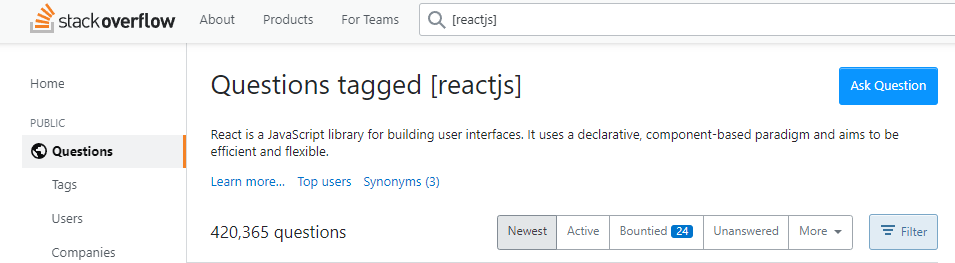
\includegraphics[width=10cm,height=10cm,keepaspectratio]{stack overflow.png}
    \end{center}
    \caption[คำถามใน Stack overflow]{คำถามใน Stack overflow}
    \label{fig:คำถามใน Stack overflow (ค้นหาเมื่อ 14/10/2565)}
\end{figure}

\subsection{Nest และ TypeScript}
Nest เป็น Framework ของ Node.js ในการจัดการ Appliction ฝั่ง Backend โดย Nest จะใช้งานร่วมกับ TypeScript 
โดย Nest นั้นสามารถขยายได้ง่าย มีการทำงานเป็นระบบแยกเป็นส่วนๆได้ ทำให้ง่ายต่อการจัดการ และการใช้ภาษา TypeScript นั้นทำให้เขียนโค้ดได้
functional มีการกำหนดชนิดของตัวแปรชัดเจนทำให้การจัดการกับข้อมูลที่เข้ามาและส่งไปได้ถูกต้อง และหาบัคนั้นได้ง่าย

\subsection{PostgreSQL และ Firebase Cloud Storage}
PostgreSQL นั้นมีการจัดการ และจัดเก็บข้อมูลในรูปแบบ structure ซึ่งเหมาะในการจัดการระบบที่ต้องการความแม่นยำ และถูกต้อง
แต่ไม่สามารถเก็บภาพ หรือวีดีโอได้ ทำให้เราต้องใช้Firebase Clound Storage เข้ามาช่วยโดยทำการอัพโหลดรูป หรือวีดีโอขึ้นไปเก็บไว้บน Firebase และรับลิ๊งของรูปภาพหรือวีดีโอ
มาเก็บไว้ใน PostgreSQL Database เพื่อในมาเรียกใช้งานภาพหลัง เนื่องจากในแพรตฟอร์มนี้จะมีการเก็บรูปภาพหลักกฐานการแข่งขันด้วยทำให้ต้องมีระบบส่วนนี้เข้ามาลองรับการใช้งาน

\begin{figure}[h]
    \begin{center}
    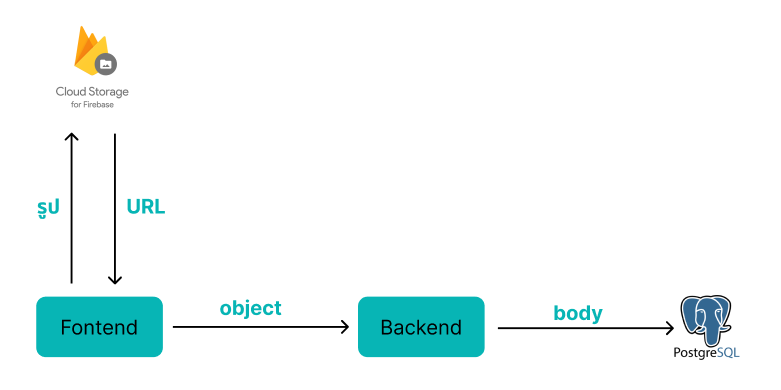
\includegraphics[width=10cm,height=10cm,keepaspectratio]{firebase.png}
    \end{center}
    \caption[การจัดเก็บรูปภาพ]{การจัดเก็บรูปภาพ}
    \label{fig:การจัดเก็บรูปภาพ}
\end{figure}

\subsection{Docker}
Docker ใช้ในการทำ Docker Images และในไปลงใน Docker Container เพื่อในไป Deploy โดยข้อดีของการใช้ Docker คือเราสามารถ  Container ที่เดียวสามารถ Deploy ได้ทุกที่ที่มี Docker รันอยู่โดยไม่ต้องกลัวว่าจะไม่สามารถรันได้
และ ง่ายกับการขยายโดยทำเป็น microservices แยกเป็นแต่ละ Docker Container ในโปรเจคนี้จะแยกออกเป็นสอง Container ได้แก่  Fontend และ Backend 

\section{\ifenglish%
\ifcpe CPE \else ISNE \fi knowledge used, applied, or integrated in this project
\else%
ความรู้ตามหลักสูตรซึ่งถูกนำมาใช้หรือบูรณาการในโครงงาน
\fi
}

\begin{enumerate}
    \item Database: การออกแบบดาต้าเบส
    \item IT Infra and Cloud Tech: การใช้ Docker ในการทำ Docker Image และ Container เพื่อในไปใช้ Deploy
\end{enumerate}

\section{\ifenglish%
Extracurricular knowledge used, applied, or integrated in this project
\else%
ความรู้นอกหลักสูตรซึ่งถูกนำมาใช้หรือบูรณาการในโครงงาน
\fi
}

\begin{enumerate}
    \item ภาษาโปรแกรมมิ่งสำหรับทำเว็ปแอพพลิเคชัน และ Framework ที่มีประสิทธิภาพในการใช้งานเพื่อเพิ่มความสะดวก และรวดเร็วในการพัฒนาเว็ปแอพพลิเคชั่น
    \item การจัดเก็บรูปภาพ และการดึงมาใช้ร่วมกับการใช้ฐานข้อมูลแบบSQL โดยการใช้ Cloud มาเป็นตัวช่วย
\end{enumerate}

\chapter{\ifproject%
\ifenglish Project Structure and Methodology\else โครงสร้างและขั้นตอนการทำงาน\fi
\else%
\ifenglish Project Structure\else โครงสร้างของโครงงาน\fi
\fi
}

ในบทนี้จะกล่าวถึงหลักการ และการออกแบบระบบ

\makeatletter

% \renewcommand\section{\@startsection {section}{1}{\z@}%
%                                    {13.5ex \@plus -1ex \@minus -.2ex}%
%                                    {2.3ex \@plus.2ex}%
%                                    {\normalfont\large\bfseries}}

\makeatother
%\vspace{2ex}
% \titleformat{\section}{\normalfont\bfseries}{\thesection}{1em}{}
% \titlespacing*{\section}{0pt}{10ex}{0pt}

\section{โครงสร้างของเว็บไซต์}
โปรเจคนี้จะแบ่งออกเป็น 3 ส่วน ตามรูปที่ 3.1
\begin{enumerate}
  \item Fontend - ใช้ React ในการจัดการหน้าเว็ปไซต์
  \item Backend - ใช้ Nest เป็นตัวกลางในการสื่อสารระหว่าง Fontend และ Database ด้วย API
  \item Database - ใช้การเก็บข้อมูลแบบ SQL โดยใช้ PostgreSQL และใช้ Firebase Cloud Storage ในการเก็บรูปภาพจากการอัพโหลด
\end{enumerate}


\begin{figure}[h]
  \begin{center}
  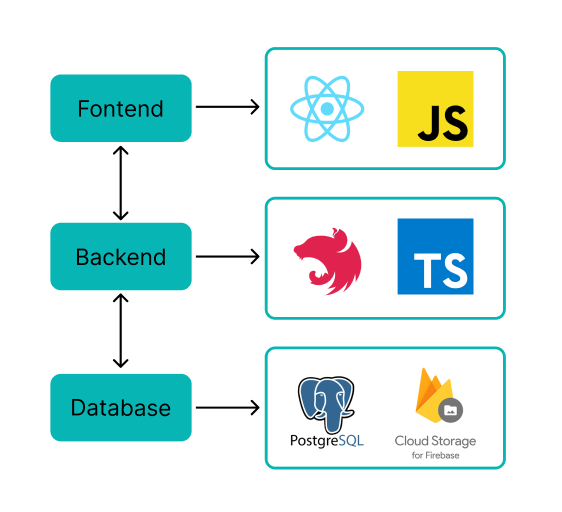
\includegraphics[width=6cm,height=6cm,keepaspectratio]{SWA.png}
  \end{center}
  \caption[โครงสร้างของเว็บไซต์]{โครงสร้างของเว็บไซต์}
  \label{fig:โครงสร้างของเว็บไซต์}
\end{figure}

\section{ฟีเจอร์}
\subsection{ฟีเจอร์การใช้งานของผู้เล่น}
การใช้งานในฝั่งผู้เล่นจะมีระบบหลักๆ ดังนี้
\begin{enumerate}
  \item ระบบสร้างทีม - ใช้สร้างทีมเพื่อเข้าร่วมการแข่งขันทัวร์นาเมนต์ต่างๆ โดยจะสร้างทีมเป็นของแต่ละเกมที่ต้องการแข่งแยกกัน เช่น ทีมValorant ก็จะใช้ลงทัวร์นาเมนต์ได้แค่เกม Valorant เท่านั้น
  \item ระบบจัดการทีม - ใช้จัดการในการเปลี่ยนชื่อ จัดการคนในทีม รับคนเข้าทีม และแสดงประวัติการเล่นของทีม
  \item ระบบจัดการโปรไฟล์ - ใช้จัดการโปรไฟล์เปลี่ยนชื่อ แสดงข้อมูลการเข้าร่วมแข่ง และทีมที่อยู่
  \item ระบบเลือก และสมัครทัวร์นาเมนต์ - เลือกทัวร์นาเมนต์ที่ต้องการแข่งขั้นสามารถดูรายละเอียด เลือกเกมที่ต้องการ และสมัครเข้าร่วมการแข่งขันได้
\end{enumerate}

\subsection{ฟีเจอร์การใช้งานของผู้จัดงาน}
การใช้งานในฝั่งผู้จัดการจะมีระบบหลักๆ ดังนี้
\begin{enumerate}
  \item ระบบสร้างจัดการทัวร์นาเมนต์ - ใช้สร้างทัวร์นาเมต์กำหนดรายระเอียดการแข่ง กฎกติกา เวลาแข่ง และรูปหน้าปกทัวร์นาเมนต์
  \item ระบบเดชบอร์ดในการจัดการทัวร์นาเมนต์ - ใช้ในการจัดการทัวร์นาเมนต์ผลแพ้ชนะ และเช็คหลักฐานการแข่งของแต่ละทีม
  \item ระบบจัดตารางแข่ง - โดยระบบจะนำผู้เล่นที่มาสมัครเข้าทัวร์นาเมนต์นั้นๆมาสุ่มเรียงเข้าตารางให้ และอัพเดตตารางการแข่งขันเมื่อผลการแข่งขันมีการปรับเปลี่ยน
\end{enumerate}

\begin{figure}[h]
  \begin{center}
  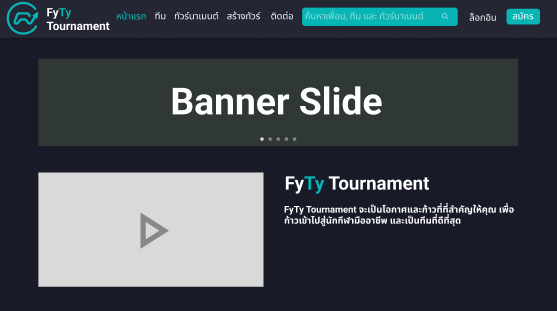
\includegraphics[width=10cm,height=6cm,keepaspectratio]{homebf.png}
  \end{center}
  \caption[หน้าแรกของระบบที่ยังไม่ได้ล็อกอิน]{หน้าแรกของระบบที่ยังไม่ได้ล็อกอิน}
  \label{fig:หน้าแรกของระบบที่ยังไม่ได้ล็อกอิน}
\end{figure}

\begin{figure}[h]
  \begin{center}
  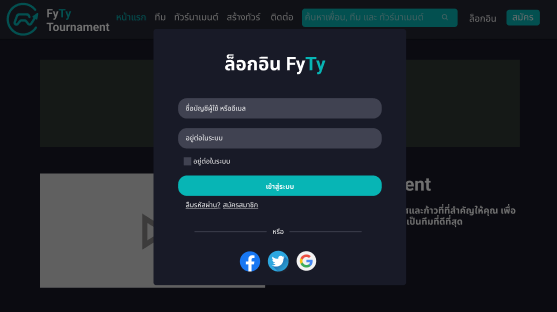
\includegraphics[width=10cm,height=6cm,keepaspectratio]{login.png}
  \end{center}
  \caption[หน้าล็อกอิน]{หน้าล็อกอิน}
  \label{fig:หน้าล็อกอิน}
\end{figure}

\begin{figure}[h]
  \begin{center}
  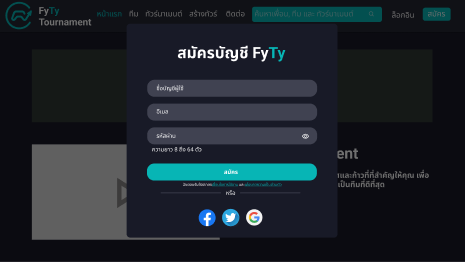
\includegraphics[width=10cm,height=6cm,keepaspectratio]{reg.png}
  \end{center}
  \caption[หน้าสมัคร]{หน้าสมัคร}
  \label{fig:หน้าสมัคร}
\end{figure}

\begin{figure}[h]
  \begin{center}
  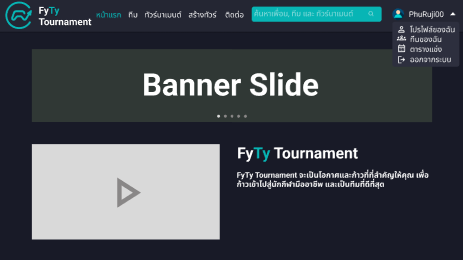
\includegraphics[width=10cm,height=6cm,keepaspectratio]{homeaf.png}
  \end{center}
  \caption[หน้าแรกของระบบหลังล็อกอิน]{หน้าแรกของระบบหลังล็อกอิน}
  \label{fig:หน้าแรกของระบบหลังล็อกอิน}
\end{figure}

\begin{figure}[h]
  \begin{center}
  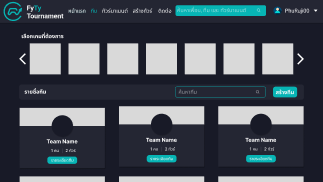
\includegraphics[width=10cm,height=6cm,keepaspectratio]{allteam.png}
  \end{center}
  \caption[หน้าทีมทั้งหมด]{หน้าทีมทั้งหมด}
  \label{fig:หน้าทีมทั้งหมด}
\end{figure}

\begin{figure}[h]
  \begin{center}
  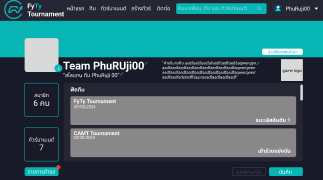
\includegraphics[width=10cm,height=6cm,keepaspectratio]{teamDetail.png}
  \end{center}
  \caption[หน้ารายละเอียดทีม และจัดการทีม]{หน้ารายละเอียดทีม และจัดการทีม}
  \label{fig:หน้ารายละเอียดทีม และจัดการทีม}
\end{figure}

\begin{figure}[h]
  \begin{center}
  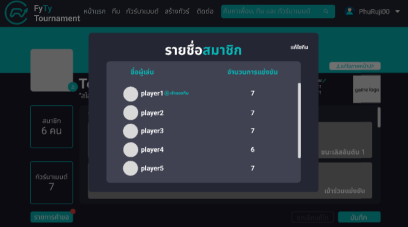
\includegraphics[width=10cm,height=6cm,keepaspectratio]{member.png}
  \end{center}
  \caption[หน้ารายละเอียดทีม และจัดการทีม(สมาชิกทีม)]{หน้ารายละเอียดทีม และจัดการทีม(สมาชิกทีม)}
  \label{fig:หน้ารายละเอียดทีม และจัดการทีม(สมาชิกทีม)}
\end{figure}

\begin{figure}[h]
  \begin{center}
  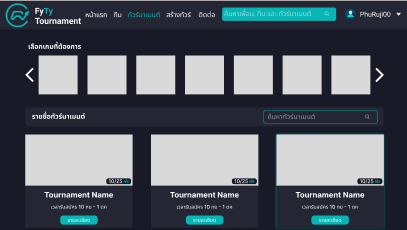
\includegraphics[width=10cm,height=6cm,keepaspectratio]{allTour.png}
  \end{center}
  \caption[หน้าทัวร์นาเมนต์ทั้งหมด]{หน้าทัวร์นาเมนต์ทั้งหมด}
  \label{fig:หน้าทัวร์นาเมนต์ทั้งหมด}
\end{figure}

\begin{figure}[h]
  \begin{center}
  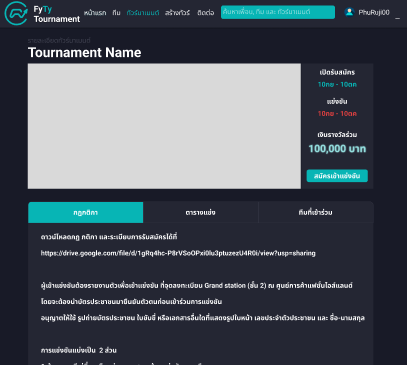
\includegraphics[width=10cm,height=10cm,keepaspectratio]{tourRule.png}
  \end{center}
  \caption[หน้ารายละเอียดทัวร์นาเมนต์(กฎกติกา)]{หน้ารายละเอียดทัวร์นาเมนต์(กฎกติกา)}
  \label{fig:หน้ารายละเอียดทัวร์นาเมนต์(กฎกติกา)}
\end{figure}

\begin{figure}[h]
  \begin{center}
  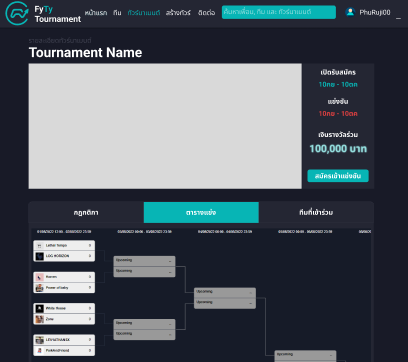
\includegraphics[width=10cm,height=10cm,keepaspectratio]{tourBac.png}
  \end{center}
  \caption[หน้ารายละเอียดทัวร์นาเมนต์(ตารางแข่ง)]{หน้ารายละเอียดทัวร์นาเมนต์(ตารางแข่ง)}
  \label{fig:หน้ารายละเอียดทัวร์นาเมนต์(ตารางแข่ง)}
\end{figure}

\begin{figure}[h]
  \begin{center}
  \includegraphics[width=10cm,height=10cm,keepaspectratio]{TourTeam.png}
  \end{center}
  \caption[หน้ารายละเอียดทัวร์นาเมนต์(ทีมที่สมัคร)]{หน้ารายละเอียดทัวร์นาเมนต์(ทีมที่สมัคร)}
  \label{fig:หน้ารายละเอียดทัวร์นาเมนต์(ทีมที่สมัคร)}
\end{figure}

\chapter{\ifenglish System Evaluation\else การประเมินระบบ\fi}

ในบทนี้จะทดสอบเกี่ยวกับการทำงานในฟังก์ชันหลักๆ

\section{การเข้าร่วมแข่งขัน}
การที่จะเข้าร่วมการแข่งขันได้นั้นต้องมีทีมที่ตรงกับเกมนั้นก่อน และต้องมีสมาชิกมากกว่าขั้นต่ำของจำนวนผู้เล่นขั้นต่ำของเกมนั้นๆ เช่น
เกม Valorant ที่ต้องมีผู้เล่น 5 การที่จะเข้าร่วมทัวร์นาเมนต์เกมนี้ได้ต้องมีทีมของเกม Valorant และมีผู้เล่นตั้งแต่ 5คนขึ้นไปถึงจะสามารถสมัครแข่งได้
\section{ตารางแข่ง}
สามารถสุ่มผู้เล่นลงตารางเวลาแข่งได้ครบและถูกต้อง มีการแสดงผลจากการเปลี่ยนแปลงผลการแข่งขันได้อัตโนมัติและถูกต้อง
\section{ระบบเดชบอร์ดในการจัดการทัวร์นาเมนต์}
สามารถใช้งานได้ครอบคลุมสามารถจัดการได้ในที่เดียวมีการแสดงผลที่ตรงกตามข้อมูลที่ได้มา
\section{ประวัติการแข่งของทีมและผู้เล่น}
แสงดงประวัติได้ถูกต้องและครบถ้วน

\ifproject
\include{chapters/conclusion}
\fi

\bibliography{sampleReport}

\ifproject
\normalspacing
\appendix
\include{chapters/appendix}

%% Display glossary (optional) -- need glossary option.
\ifglossary\glossarypage\fi

%% Display index (optional) -- need idx option.
\ifindex\indexpage\fi

\begin{biosketch}
\begin{center}
  \includegraphics[width=1.5in]{mugshot.jpg}
\end{center}
Your biosketch goes here. Make sure it sits inside
the \texttt{biosketch} environment.
\end{biosketch}
\fi % \ifproject
\end{document}

